\documentclass[letterpaper]{article}
\usepackage[submission]{aaai2027}
\usepackage[hyphens]{url}
\usepackage{graphicx}
\urlstyle{rm}
\def\UrlFont{\rm}
\usepackage{natbib}
\usepackage{caption}
\frenchspacing
\usepackage{amsmath,amssymb,amsfonts}
\usepackage{booktabs}
\usepackage{multirow}
\usepackage{array}
\usepackage{tabularx}
\usepackage{colortbl}
\usepackage{xspace}
\usepackage{algorithm}
\usepackage{algorithmic}
\pdfinfo{/TemplateVersion (2027.1)}
\setcounter{secnumdepth}{2}
\definecolor{headerrow}{RGB}{216,231,252}
\definecolor{rghlirow}{RGB}{211,242,222}
\definecolor{controlrow}{RGB}{222,241,252}
\definecolor{cautionrow}{RGB}{255,236,190}
\definecolor{corerow}{RGB}{238,226,251}
\definecolor{gridline}{RGB}{112,139,176}
\arrayrulecolor{gridline}
\newcolumntype{Y}{>{\raggedright\arraybackslash}X}
\newcommand{\tblhdr}{\rowcolor{headerrow}}
\newcommand{\method}{\emph{residual-guided hypothesis-language induction}\xspace}
\newcommand{\methodshort}{\textsc{RG-HLI}\xspace}
\newcommand{\uhk}{\textsc{UHK}\xspace}
\newcommand{\mek}{\textsc{MEK}\xspace}
\newcommand{\react}{\textsc{ReAct}\xspace}
\newcommand{\codeact}{CodeAct\xspace}
\newcommand{\gptmini}{GPT-4o-mini\xspace}
\newcommand{\gptfour}{GPT-4o\xspace}
\newcommand{\deepseek}{DeepSeek\xspace}
\newcommand{\hms}{\ensuremath{\mathrm{HMS}}\xspace}
\newcommand{\sa}{\ensuremath{\mathrm{SA}}\xspace}
\newcommand{\sr}{\ensuremath{\mathrm{SR}}\xspace}
\newcommand{\ver}{\ensuremath{\mathrm{VER}}\xspace}
\newcommand{\fileid}[1]{\texttt{\small\detokenize{#1}}}
\title{Supplementary Material for\\ Residual-Guided Hypothesis Language Induction for Scientific Reasoning with Small Language Models}
\author{Anonymous Submission}
\affiliations{}
\begin{document}
\onecolumn

\begin{center}
{\Large\bfseries Supplementary Material}\\[3pt]
{\large\bfseries Residual-Guided Hypothesis Language Induction for Scientific
Reasoning with Small Language Models}\\[3pt]
{\normalsize Anonymous Submission}
\end{center}

\section*{Appendix: Experimental Details and Ablations}

This appendix is deliberately more explicit than the main text. The main paper
reports compact benchmark-level claims; the appendix separates three questions:
which complete runs support the headline table, how matched reasoning controls
and uncertainty are measured, and how frozen-transfer and multi-step audits
isolate residual-conditioned language growth.

\begin{table}[!htbp]
\centering
\small
\begin{tabularx}{0.96\textwidth}{|l|c|c|Y|Y|}
\hline
\tblhdr
Benchmark & Tasks & Core model & Evaluator & Result \\
\hline
DiscoveryBench & 239 & \gptmini & HMS judge & 28.70 HMS; 34.56 Cons-HMS \\
\hline
NewtonBench & 324 & \gptmini & symbolic-law judge & 49.38\% SA-all; 66.67\% SA-answered \\
\hline
UltraHorizon & 96 & \gptmini & environment score & 51.04 strict \\
\hline
\end{tabularx}
\caption{Complete-run audit used for the headline results. Each row uses the
benchmark-native evaluator.}
\label{tab:appendix_fullrun_audit}
\end{table}

For NewtonBench, the complete run answered 240 of 324 tasks and abstained on
84, yielding 74.1\% coverage and a 25.9\% abstention rate. SA-all assigns zero
to abstentions; SA-answered is computed only over the 240 submitted laws. The
49.38/66.67 row is the retained single-pass evaluator result and does not use
selective rejudging. This canonical benchmark run uses the frozen typed
executable kernel with development-time promotion gates disabled; it is
therefore evidence for per-task hypothesis construction, not for the promotion
mechanism. Frozen-transfer and multi-step experiments below evaluate promotion
separately.

\subsection*{External Reasoning Baselines}

Matched non-\methodshort baselines are useful only when they are run on the same
complete benchmark set. Table~\ref{tab:external_reasoning} reports completed
DiscoveryBench controls that satisfy this condition. They use the same
\gptmini core, task set, and native evaluator as the corresponding headline
run, but they do not expose \methodshort typed state, residual objects,
answer-slot closure, or operator promotion.

\begin{table}[!htbp]
\centering
\small
\begin{tabularx}{0.90\textwidth}{|l|c|c|Y|}
\hline
\tblhdr
Method & Tasks & HMS & Interface \\
\hline
\rowcolor{controlrow}
Direct \gptmini & 239 & 9.54 & single prompt \\
\hline
\rowcolor{controlrow}
\react \gptmini & 239 & 11.68 & thought-check trace \\
\hline
\rowcolor{controlrow}
CodeAct \gptmini & 239 & 12.31 & executed summaries \\
\hline
\rowcolor{rghlirow}
\methodshort \gptmini & 239 & 28.70 & typed language state \\
\hline
\end{tabularx}
\caption{Matched external reasoning controls on DiscoveryBench. All rows use
the same task set and HMS evaluator.}
\label{tab:external_reasoning}
\end{table}

The gap is not evidence that ordinary prompting is useless. It shows that, under
the DiscoveryBench HMS contract, longer traces and one-pass executed summaries
do not reproduce the effect of typed answer construction and
residual-conditioned rendering.

\subsection*{Matched-Control Uncertainty}

The complete DiscoveryBench controls admit a task-paired comparison because
all four methods use the same 239 rows and evaluator. Table~\ref{tab:paired_db}
reports the gain of \methodshort over each external control. All three
intervals exclude zero; this is stronger evidence than comparing only
aggregate point estimates.

\begin{table}[!htbp]
\centering
\small
\begin{tabularx}{0.92\textwidth}{|l|c|c|c|}
\hline
\tblhdr
Control & Control HMS & \methodshort gain & 95\% interval \\
\hline
\rowcolor{controlrow}
Direct & 9.54 & +19.16 & [12.81, 25.68] \\
\hline
\rowcolor{controlrow}
\react & 11.68 & +17.01 & [10.99, 23.12] \\
\hline
\rowcolor{controlrow}
CodeAct & 12.31 & +16.39 & [9.87, 23.01] \\
\hline
\end{tabularx}
\caption{Paired DiscoveryBench gains. Intervals use 10,000 nonparametric
bootstrap draws over common task rows with seed 20260721.}
\label{tab:paired_db}
\end{table}

\subsection*{Operator Reuse in the Frozen Language}

The retained DiscoveryBench trace records which named operator family produced
each final artifact. Table~\ref{tab:operator_reuse} includes every named family
selected on at least three tasks. The same family is reused across task rows
and, in several cases, across scientific domains. These counts describe use of
the frozen language; causal benefit is evaluated separately by the paired
controls above and the frozen-transfer experiment below. Every family in this
table is selected and task-parameterized from frozen $L^\star$; none is
synthesized or promoted during reported evaluation.

\begin{table}[!htbp]
\centering
\small
\begin{tabularx}{0.88\textwidth}{|Y|c|c|}
\hline
\tblhdr
Operator family & Tasks selected & Domains \\
\hline
answer plan & 39 & 5 \\
\hline
universal slot closure & 34 & 3 \\
\hline
estimand synthesizer & 25 & 3 \\
\hline
evidence contract & 25 & 4 \\
\hline
contrastive world & 3 & 2 \\
\hline
slot contract & 3 & 2 \\
\hline
\end{tabularx}
\caption{Reuse of selected, task-parameterized operator families in the
complete 239-task DiscoveryBench run. Domain counts use the benchmark metadata
taxonomy.}
\label{tab:operator_reuse}
\end{table}

\subsection*{Shared Cross-Benchmark Interface}

The implementation necessarily exposes different observations---tables,
symbolic-law rows, and interactive trajectories---but the learning object is
unchanged: typed hypotheses, executable validation, residual classes, and
held-out operator promotion.  Table~\ref{tab:shared_loop} makes this boundary
explicit.

\begin{table}[!htbp]
\centering
\small
\begin{tabularx}{0.96\textwidth}{|l|Y|Y|Y|}
\hline
\tblhdr
Benchmark & Observation exposed to the kernel & Residual object & Promotable operator class \\
\hline
DiscoveryBench & tables, text snippets, requested scientific claim & missing role, wrong denominator, wrong answer facet & answer-slot closure, evidence renderer, consistency check \\
\hline
NewtonBench & numerical rows, candidate variables, target expression & wrong exponent, constant, transform, or abstention & executable probe, symbolic fit, unit-compatible verifier \\
\hline
UltraHorizon & trajectory, action log, rule feedback, replay state & failed replay, local invariant, missing exploration evidence & exploration policy, replay validator, temporal abstraction \\
\hline
\end{tabularx}
\caption{How the same residual-to-operator loop appears in the three benchmark
families. These are not separate solvers; they are domain-specific observations
fed into the same state machine.}
\label{tab:shared_loop}
\end{table}

\subsection*{Typed Prompt and Operator Interface}

The benchmark-facing prompts are intentionally narrow. The model is not asked
to ``think longer'' or to invent a complete answer in free text. Each call must
return one typed object that can be executed, checked, or converted into a
residual. Table~\ref{tab:prompt_contracts} gives the prompt contracts used by
the kernel. The same contract structure is used across all three benchmarks;
only the observation serializer and native validator differ.

\begin{table}[!htbp]
\centering
\small
\begin{tabularx}{0.96\textwidth}{|l|Y|Y|Y|}
\hline
\tblhdr
Call & Input state & Required output & Rejection rule \\
\hline
Contract compiler & task observation, available tools, current $L^\star$ & roles, admissible answer form, measurable holes, validator names & missing target role or non-executable hole \\
\hline
Probe writer & contract, hole, evidence table or trajectory & short executable measurement with declared inputs and expected type & code fails, reads forbidden fields, or returns wrong type \\
\hline
Hypothesis composer & closed holes, evidence objects, active operators & artifact $h$: law, claim, program, or rule mapping & artifact cannot be replayed or violates contract \\
\hline
Residual compiler & failed validation trace & typed residual $(\tau,\ell,c,e,v)$ & free-text criticism without location, evidence, and failed validator \\
\hline
Operator proposer & recurring residual class $R_k$ and held-out tasks & candidate operator $o^\star$ with scope, cost, and validator hooks & no residual class closed, no executable hook, or excessive complexity \\
\hline
\end{tabularx}
\caption{Prompt contracts used by \methodshort. Each prompt returns a typed
object with an attached validation path rather than an unconstrained chain of
thought.}
\label{tab:prompt_contracts}
\end{table}

Operators are added through a single interface. The implementation may contain
benchmark adapters, but an accepted operator must expose the same fields:
scope, precondition, executable transform, evidence update, residual update,
complexity cost, and promotion evidence. In simplified form, an operator is
accepted only if it satisfies the following contract:

\begin{quote}
\small
\ttfamily
operator.id: stable name;\\
operator.scope: residual types and artifact slots where it is admissible;\\
operator.precondition(state, contract) -> bool;\\
operator.apply(state, contract) -> artifact/evidence/residual update;\\
operator.cost -> $\beta K_o$, where $K_o=\log(1+n_{\mathrm{AST}})$ and $\beta=10^{-3}$;\\
operator.validators -> executable checks that must pass;\\
promote iff heldout\_utility\_gain(operator) $-\beta K_o>0$.
\end{quote}

All promotable operators are serialized into the same executable Python
intermediate representation before validation; declarative schemas and
policies are first compiled to this representation. Thus,
$n_{\mathrm{AST}}$ always counts nodes in one canonical executable form.
Predefined interface components are part of $L_0$ and are not retrospectively
charged as promoted operators. We fixed $\beta=10^{-3}$ before the reported
trajectory and did not tune it on transfer interfaces.

This interface is the main difference between residual-conditioned language
growth and ordinary prompt iteration. A failed hypothesis does not merely
produce another instruction for the model. It produces a typed residual with a
location and failed validator; only repeated residuals can ask for a new
operator, and the operator is not retained unless it improves held-out tasks
under the same validator stack.

\begin{algorithm}[H]
\caption{Per-task executable search in a frozen language}
\label{alg:frozen_search}
\begin{algorithmic}[1]
\REQUIRE task $x$, frozen language $L^\star=(\mathcal{Y},\mathcal{O})$, budget $B$
\ENSURE rendered answer $R_x(h^\star)$
\STATE compile evidence contract $C_x$ and initialize context $\mathcal{M}_x$
\FOR{$t=1,\ldots,B$}
  \STATE select type-admissible operator $O_t\in\mathcal{O}$
  \STATE execute $O_t(\mathcal{M}_x,x)$ to obtain $(h,e,\rho,\Delta\mathcal{M})$
  \STATE write evidence, closed holes, and any residual to $\mathcal{M}_x$
  \STATE update $h^\star$ using evidence, coverage, validation, and $K_h$
\ENDFOR
\STATE validate and render $R_x(h^\star)$
\STATE log residuals for audit without changing $L^\star$
\RETURN $R_x(h^\star)$
\end{algorithmic}
\end{algorithm}

Residual clustering is rule-based in the reported audit. The canonical
signature is
\[
 \sigma(\rho)=
 (\tau_\rho,\operatorname{canon}(\ell_\rho),
 \operatorname{role}(c_\rho),\operatorname{geometry}(e_\rho)),
\]
where canonicalization removes task-local names and function signatures, and
evidence geometry records typed properties such as positive/log-structured or
positive/non-log-structured data. We set $\rho_i\sim\rho_j$ iff their signatures
match exactly and call a class recurrent when it contains at least
$m_{\min}=2$ source residuals. For promotion,
$r(O')=\sum_{x\in\mathcal{D}_{prom}}
\mathbb{1}[U_x(h^\star_{O'})>U_x(h^\star)]$ and the reported trajectory
requires $r(O')\geq r_{\min}=1$. Source, promotion, and transfer interfaces are
disjoint; transfer utility is recorded only after the decision and cannot
change it.

\begin{algorithm}[H]
\caption{Residual-conditioned language growth on development tasks}
\label{alg:language_growth}
\begin{algorithmic}[1]
\REQUIRE language $L_t$, disjoint sets $\mathcal{D}_{ind}$,
$\mathcal{D}_{prom}$, and $\mathcal{D}_{transfer}$
\ENSURE $L_{t+1}$
\STATE $L_{\mathrm{new}}\leftarrow L_t$
\STATE solve $\mathcal{D}_{ind}$ with Algorithm~\ref{alg:frozen_search} and collect residuals
\STATE group residuals by canonical signature $\sigma(\rho)$
\FOR{each recurrent residual class $\mathcal{R}_k$}
  \STATE propose executable operator $O'$ with declared scope and validators
  \IF{$O'$ fails typing, sandbox execution, or validator checks}
    \STATE discard $O'$ and continue
  \ENDIF
  \STATE measure held-out utility gain $G(O')$ on $\mathcal{D}_{prom}$
  \STATE compute $K_o(O')=\log(1+n_{\mathrm{AST}}(O'))$
  \IF{$G(O')-\beta K_o(O')>0$ and $r(O')\geq r_{\min}$}
    \STATE $L_{\mathrm{new}}\leftarrow L_{\mathrm{new}}\cup\{O'\}$
  \ENDIF
\ENDFOR
\STATE freeze $L_{t+1}\leftarrow L_{\mathrm{new}}$
\STATE audit transfer on $\mathcal{D}_{transfer}$ without updating $L_{t+1}$
\RETURN $L_{t+1}$
\end{algorithmic}
\end{algorithm}

\subsection*{State-Mutation Invariants}

The two algorithms expose all persistent writes. A proposal may be stochastic,
but the transition is admitted only after deterministic type, execution, and
validator checks. Table~\ref{tab:state_mutation_invariants} makes the mutation
boundary explicit: task-local search can enrich evidence and close holes,
whereas only the development-time promotion procedure can change the operator
language. Native benchmark scores are terminal observations and have no write
path into either state.

\begin{table}[!htbp]
\centering
\small
\begin{tabularx}{0.96\textwidth}{|l|Y|Y|}
\hline
\tblhdr
Invariant & Admissible write & Rejected transition \\
\hline
Type preservation & close a hole with an artifact of its declared type & missing type, incompatible slot, or invalid renderer \\
\hline
Evidence monotonicity & append a probe result with source and validator trace & overwrite retained evidence or read a forbidden field \\
\hline
Executable closure & commit only sandboxed code or a compiled declarative transform & free-form repair with no executable semantics \\
\hline
Frozen evaluation & select and parameterize operators already in $L^\star$ & synthesize or promote from a reported test row \\
\hline
Score isolation & emit the final rendered artifact to the native evaluator & use benchmark score or gold output as an internal update \\
\hline
\end{tabularx}
\caption{Mutation invariants enforced by the shared implementation. ``Reject''
means that the attempted transition is converted into a typed residual and the
previous valid state is retained.}
\label{tab:state_mutation_invariants}
\end{table}

These constraints also identify the source of every capability change. Better
search with fixed $L^\star$ is an inference effect; a new constructible
artifact family requires a separately logged promotion event. This distinction
is what lets the mechanism audit attribute transfer to language growth rather
than to an unrecorded prompt or state mutation.

\subsection*{Worked Hypothesis Construction Trace}

Figure~\ref{fig:concrete_language_growth} shows the intended granularity of a single
DiscoveryBench-style task. The model is not asked to guess the final scientific
sentence in one pass. It first commits to a typed contract, then executable
measurements close slots, and only the rendered artifact is sent to the native
evaluator. A failure is not stored as prose feedback; it is stored as the
violated slot or validator.

\begin{figure}[!htbp]
\centering
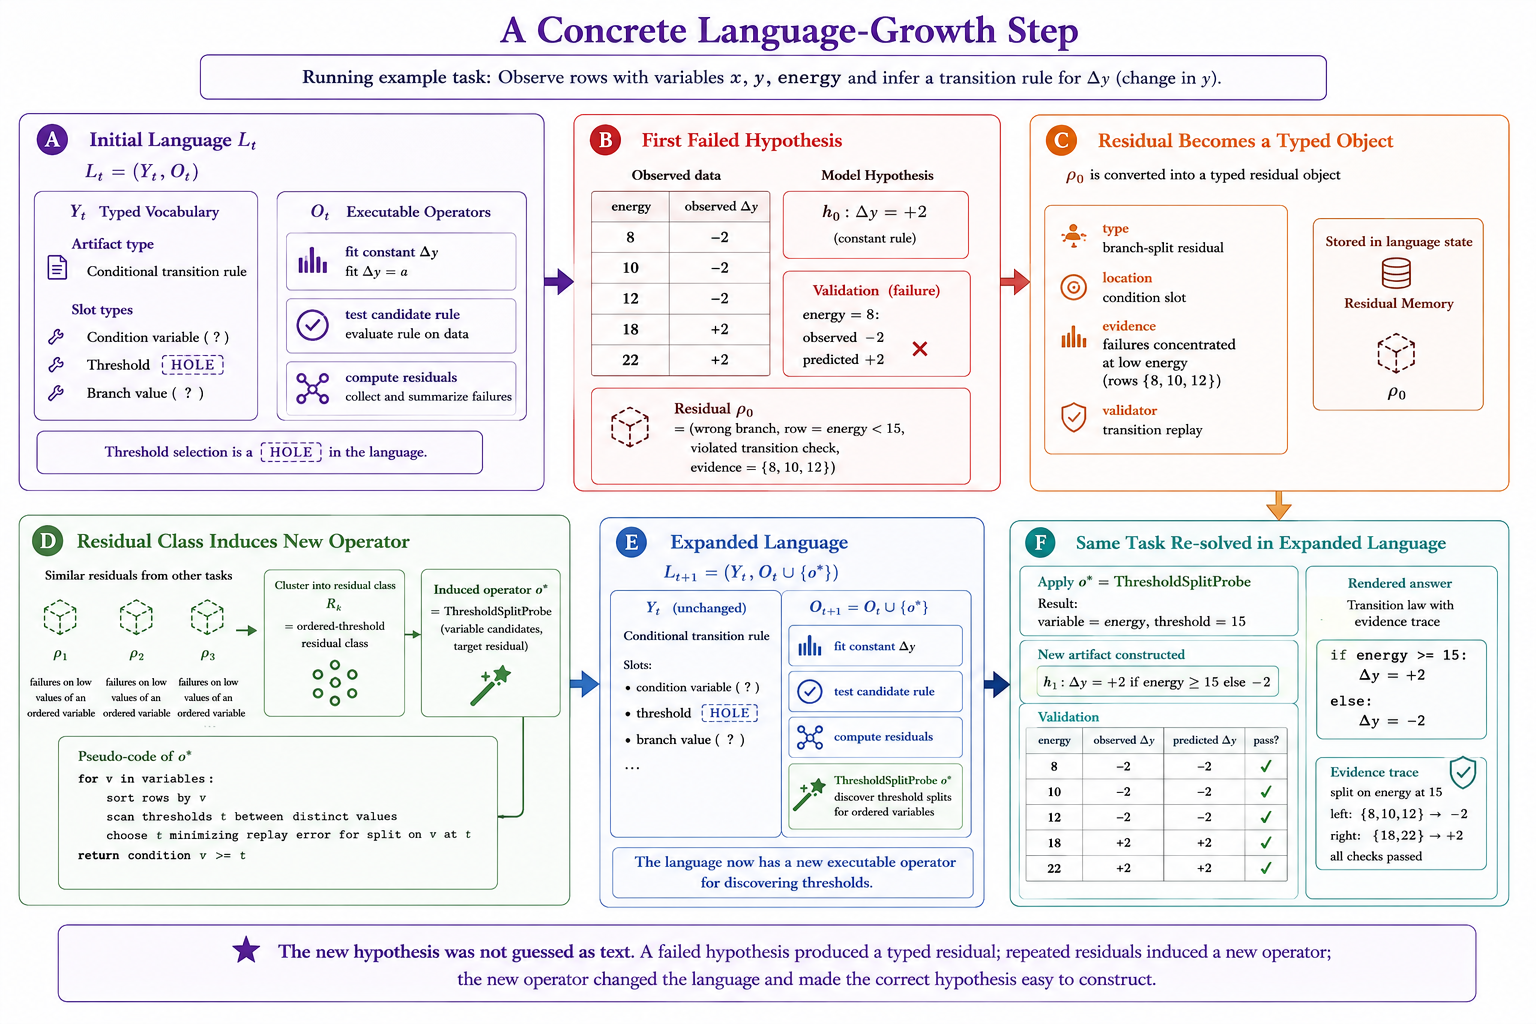
\includegraphics[width=0.84\textwidth]{paper_assets/figures/concrete_language_growth_step.png}
\caption{Worked construction of a language-growth step, included to expose the
typed objects rather than as a benchmark result. A failed constant transition
hypothesis is converted into a typed residual; repeated residuals induce a
threshold-split operator; the expanded language then makes the correct
conditional transition artifact easy to construct and validate.}
\label{fig:concrete_language_growth}
\end{figure}

\subsection*{Retained UltraHorizon Trace}

The following record is a strict Seq episode retained from the UltraHorizon
evaluation artifact. It makes the long-horizon interface concrete: the system
must infer a program from interventions, preserve the resulting rules across a
50-step interaction horizon, and finally render the rules for the paper-style
judge.

\begin{figure}[!htbp]
\centering
\fcolorbox{gridline}{controlrow}{%
\begin{minipage}{0.92\textwidth}
\small
\textbf{A retained strict UltraHorizon Seq episode}\\
\rule{\linewidth}{0.25pt}\\
\textsc{First intervention.} $\mathrm{main}=\texttt{ABCDE}$ and
$\mathrm{vice}=\texttt{DECBA}$ produce $\texttt{ADBECCDBEA}$ after the first transformation.\\
\textsc{Typed trace slot.} The system records an \emph{interleave-step-parity}
rule: interleave the two strings; main leads on odd experiment steps and vice
leads on even steps.\\
\textsc{Additional executable slots.} The final program contains five rules,
including a reverse-and-shift composition, a step-indexed copy operation, a
history-dependent alphabetic sum, and a prime-step frequency replacement.\\
\textsc{Commit and verification.} $50$ observations, $27$ planning turns, and
$54$ environment actions yield all five exact rule matches under the
paper-style judge. No hint, measurement bootstrap, or fallback commit was
exercised.
\end{minipage}}
\caption{A concrete long-horizon artifact. The retained state is a typed,
replayable rule program assembled from interventions, not a prose summary of
the trajectory.}
\label{fig:uh_text_exhibit}
\end{figure}

\subsection*{Qualitative Operator-Induction Example}

The following DiscoveryBench example illustrates the intended language-growth
mechanism. A first full audit exposed repeated failures on study-design tables:
the system often measured a real effect but selected the wrong role, such as
confusing original and replication studies or measuring the complement of a
binary design variable. These errors produced a shared residual type:
\emph{study-design role closure}. The induced operator did not memorize a
dataset answer. It added a reusable repair interface: conservative aliases for
original/replication roles, paired-column completion, binary complement
closure, and contrastive rendering of the selected role.

\begin{table}[!htbp]
\centering
\small
\begin{tabularx}{0.96\textwidth}{|l|Y|}
\hline
\tblhdr
Element & Description \\
\hline
Observed failures & repeated wrong-role and wrong-complement answers in study-design tables \\
\hline
Residual object & $(\tau_\rho=\text{role-closure},\ell_\rho=\text{answer slot},c_\rho=\text{study role},e_\rho=\text{paired columns},v_\rho=\text{consistency check})$ \\
\hline
Candidate operator & close original/replication roles with conservative aliases, paired-column completion, binary complements, and contrastive rendering \\
\hline
Promotion evidence & the operator must pass held-out promotion before inclusion in the frozen language \\
\hline
Declared scope & study-design role closure; denominator alignment and nonlinear regression use separate typed interfaces \\
\hline
\end{tabularx}
\caption{Example of a residual-induced operator. The operator is described as a
repair interface over typed residuals, not as a benchmark answer template.}
\label{tab:operator_example}
\end{table}

\subsection*{Strict Frozen-Language Transfer Diagnostic}

The complete-run controls above establish benchmark-level differences, but a
second diagnostic isolates the narrower causal question: can a residual-induced
operator improve later tasks when no additional free-form search is allowed?
We use NewtonBench in its hard, \texttt{v0}, vanilla-equation setting. Two
source law interfaces (gravity and Coulomb force) are used only to produce a
recurring \texttt{dict}$\rightarrow$\texttt{float} residual class. The
induction phase classifies the residual geometry as
\texttt{positive\_log\_structured} and selects a generic
positive-monomial lattice from two contract-compatible numerical families
(monomial and additive). It stores neither source observations nor source task
identifiers; a provenance audit checks the persisted operator source for both
identifiers.

For the held-out phase, the language is frozen and evaluated on magnetic force,
Fourier law, radioactive decay, and Hooke law. $L_0$ contains the same minimal
typed execution state but disables typed priors, residual kernels,
decompose--plan--stage--recombine (DPSR), stored
candidate layers, language writes, and free-form LLM rounds. $L_1=L_0\cup
\{o^\star\}$ adds only the frozen residual-induced operator. Both conditions
receive the same 24 observations and the same train/hold-out split per task;
the operator may calibrate a scalar only from the current task's training
observations. Thus, the held-out comparison adds neither model calls nor new
operators. This diagnostic reports internal executable loss, not the official
symbolic-agreement metric.

\begin{table}[!htbp]
\centering
\small
\begin{tabularx}{0.98\textwidth}{|c|c|c|c|c|Y|}
\hline
\tblhdr
Seed & $L_0$ & selected $L_1$ & additive control & selection gain & audit \\
\hline
13 & 1.000 & 0.308 & 0.488 & 0.179 & monomial; identifiers absent \\
\hline
31 & 1.000 & 0.351 & 0.528 & 0.177 & monomial; identifiers absent \\
\hline
57 & 1.000 & 0.339 & 0.496 & 0.157 & monomial; identifiers absent \\
\hline
\rowcolor{rghlirow}
Mean & 1.000 & $0.333 \pm 0.022$ & $0.504 \pm 0.021$ & $0.171 \pm 0.012$ & 12 / 12; all audits pass \\
\hline
\end{tabularx}
\caption{Frozen residual-to-language transfer diagnostic on four held-out
NewtonBench law interfaces per split. $L_1$ contains the residual-selected
monomial operator; the control contains an additive operator generated by the
same typed compiler. Lower executable loss is better.}
\label{tab:strict_language_transfer}
\end{table}

The language trajectory is $L_0\xrightarrow{\,2\;\mathrm{residuals}\,}
L_1=L_0\cup\{o^\star\}$: each residual class is supported by two disjoint
source interfaces before the operator is quarantined, then the operator is
frozen and reused on four new interfaces. Across the three fixed splits, the
selected operator reduces held-out loss by $0.667\pm0.022$, compared with
$0.496\pm0.021$ for the type-compatible additive control. Thus, adding any
executable code helps, but residual-conditioned family selection accounts for
an additional $0.171\pm0.012$ reduction under the same held-out protocol.
All ``$\pm$'' values in Table~\ref{tab:strict_language_transfer} are sample
standard deviations over the three fixed data splits.

This diagnostic complements the headline NewtonBench SA comparison by removing
new LLM proposals and online language mutation from the held-out phase while
preserving the standard executable calibration interface. The observed
advantage is therefore attributable to the frozen language extension and its
residual-conditioned family choice, rather than a longer reasoning trace or an
additional search budget.

\subsection*{Audited Multi-Step Language Growth}

We next trace two consecutive language updates rather than evaluating a single
frozen extension. Modules are partitioned only by coarse residual geometry and
module index. Within each update, source, promotion, and transfer modules are
disjoint and use seeds 13, 31, and 57, respectively. Operator source receives
neither module identifiers nor gold laws, and transfer evaluation cannot mutate
the language. Selection follows the promotion rule in the main paper with
$K(o)=\log(1+\text{AST-nodes}(o))$ and $\beta=10^{-3}$. No official benchmark
score is used for induction or promotion.

\begin{table}[!htbp]
\centering
\small
\begin{tabularx}{0.98\textwidth}{|c|Y|c|c|c|c|}
\hline
\tblhdr
Update & Proposed operator & held-out gain & $\beta K(o)$ & net gain & transfer gain \\
\hline
\rowcolor{rghlirow}
$L_0\!\rightarrow\!L_1$ & positive-monomial lattice & 0.6055 & 0.0067 & $+0.5988$; accept & 0.5871 \\
\hline
\rowcolor{rghlirow}
$L_1\!\rightarrow\!L_2$ & positive-additive pair & 0.0142 & 0.0060 & $+0.0082$; accept & 0.0996 \\
\hline
\rowcolor{controlrow}
$L_2\!\rightarrow\!L_2$ & repeated monomial operator & 0.0000 & 0.0067 & $-0.0067$; reject & 0.0000 \\
\hline
\end{tabularx}
\caption{A complete residual-guided trajectory from $L_0$ to $L_2$. Gain is
the reduction in mean executable loss on the disjoint promotion or transfer
partition; higher is better. The final row tests whether a repeated residual
class can inflate an already sufficient language.}
\label{tab:multistep_language_growth}
\end{table}

\begin{table}[!htbp]
\centering
\small
\begin{tabularx}{0.88\textwidth}{|c|c|c|c|Y|}
\hline
\tblhdr
$\beta$ & $L_0\!\rightarrow L_1$ net & $L_1\!\rightarrow L_2$ net & duplicate net & decisions \\
\hline
$5\!\times\!10^{-4}$ & $+0.6021$ & $+0.0112$ & $-0.0033$ & accept, accept, reject \\
\hline
$10^{-3}$ & $+0.5988$ & $+0.0082$ & $-0.0067$ & accept, accept, reject \\
\hline
$2\!\times\!10^{-3}$ & $+0.5921$ & $+0.0023$ & $-0.0134$ & accept, accept, reject \\
\hline
\end{tabularx}
\caption{Post-hoc complexity sensitivity using the already measured held-out
gains. No operator is re-fit and transfer interfaces remain unused.}
\label{tab:beta_sensitivity}
\end{table}

The first operator is induced from gravity and Coulomb residuals, promoted on
magnetic-force and Fourier-law interfaces, and transferred to radioactive
decay, Hooke's law, and heat transfer. The second is induced from
underdamped-harmonic and Malus-law residuals, promoted on sound speed, and
transferred to the Bose--Einstein distribution interface. Its promotion margin
is small but positive after complexity, and the frozen operator reduces loss by
0.0996 on the unseen transfer interface. A third occurrence of the first
residual class produces the same source hash. Because it adds no marginal
held-out value, the gate leaves the language at $L_2$. Both retained sources
pass a provenance scan with zero source-task identifier matches. This trajectory
therefore exhibits the full claimed mechanism: recurring failures induce
executable structure, independently measured utility grows the language, and
the same criterion suppresses redundant growth.

\begin{figure}[!htbp]
\centering
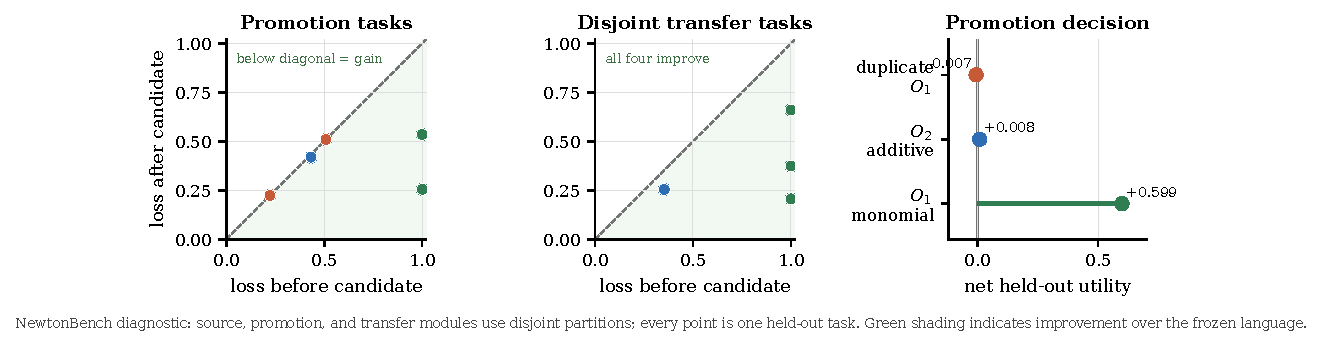
\includegraphics[width=0.94\textwidth]{paper_assets/figures/language_growth_audit.pdf}
\caption{Task-level held-out evidence for the audited language trajectory.
Each dot is an executable loss measured before and after a proposed operator;
points below the diagonal improve. Promotion and transfer partitions are
disjoint. The final panel shows that the two useful operators are admitted and
the re-proposed monomial operator is rejected by the same net-utility gate.}
\label{fig:language_growth_audit}
\end{figure}

\subsection*{Leakage and Freeze Controls}

The paper uses two distinct phases. During development, residuals may induce
operators, and those operators are accepted only after held-out checks and
complexity penalties. During the reported benchmark evaluations, the language
is frozen: the system may search within $L^\star$ for each task, but it does
not use the task's benchmark score to update $L^\star$ for later reported
tasks. Table~\ref{tab:freeze_controls} summarizes the protocol.

\begin{table}[!htbp]
\centering
\small
\begin{tabularx}{0.96\textwidth}{|l|Y|Y|}
\hline
\tblhdr
Phase & Allowed & Disallowed \\
\hline
Development induction & collect residuals, propose operators, held-out promotion & using final reported test scores as promotion targets \\
\hline
Headline evaluation & per-task search, execution, validation, rendering in frozen $L^\star$ & changing $L^\star$ from future test rows or gold labels \\
\hline
Post-run analysis & cluster failures and plan future operators & retroactively changing the reported score \\
\hline
\end{tabularx}
\caption{Protocol controls for residual-conditioned language growth.}
\label{tab:freeze_controls}
\end{table}

\subsection*{Uncertainty and Coverage}

Table~\ref{tab:bootstrap_ci} reports deterministic percentile-bootstrap
intervals over completed evaluation units. DiscoveryBench and NewtonBench
resample task rows. UltraHorizon resamples the 32 seeds independently within
each environment and then averages the three environment means. These
intervals quantify evaluation-set variation; they do not replace independent
model-call replications.

\begin{table}[!htbp]
\centering
\small
\begin{tabularx}{0.92\textwidth}{|Y|c|c|c|}
\hline
\tblhdr
Metric & Units & Estimate & 95\% interval \\
\hline
DiscoveryBench HMS & 239 tasks & 28.70 & [23.24, 34.28] \\
\hline
DiscoveryBench Cons-HMS & 239 tasks & 34.56 & [28.84, 40.33] \\
\hline
NewtonBench SA-all & 324 tasks & 49.38\% & [44.14, 54.94] \\
\hline
NewtonBench SA-answered & 240 answers & 66.67\% & [60.83, 72.50] \\
\hline
UltraHorizon strict & 96 episodes & 51.04 & [44.79, 56.88] \\
\hline
\end{tabularx}
\caption{Headline point estimates and 95\% nonparametric bootstrap intervals.
All intervals use 10,000 draws and random seed 2027.}
\label{tab:bootstrap_ci}
\end{table}

\subsection*{Operator Provenance}

The implementation distinguishes four operator origins. \emph{Predefined}
operators implement the universal typed interface and sandbox primitives.
\emph{Selected} operators are chosen from type-compatible families by residual
geometry. \emph{Parameterized} operators fit task-local constants from
observations without changing the language. \emph{Synthesized} operators are
new executable transforms proposed from recurrent development residuals and
must pass Algorithm~\ref{alg:language_growth}. Reported test tasks may select
and parameterize frozen operators, but they may not synthesize or promote new
ones. The strict transfer diagnostic specifically compares two selected,
type-compatible families while holding parameter fitting and test-time compute
fixed.

Predefined contracts, slots, verifiers, and residual interfaces constitute
$L_0$.  At evaluation time, tasks may select and parameterize operators from
frozen $L^\star$, but cannot synthesize or promote new ones.  The
positive-monomial lattice is the measured development-time extension: it is
selected by residual geometry, admitted before transfer, and evaluated on
12 held-out interface--split pairs.  Figure~\ref{fig:concrete_language_growth}
uses a threshold-split operator only to expose the same typed transition at
the level of one concrete artifact.

\subsection*{Artifact Manifest and Compute Accounting}

The machine-readable map from every reported row to its complete-run
JSON/JSONL/CSV artifact is
\path{paper_assets/evidence/evidence_index.csv}.  It
indexes the 239-task DiscoveryBench run, the 324-task NewtonBench run, the
96-episode UltraHorizon run, DiscoveryBench controls, the multi-step
trajectory, bootstrap intervals, and the complete proposal-core audits.  The
archive retains per-task outputs and evaluator decisions; no table is
reconstructed from manually selected examples. Additional proposal-core
artifacts are indexed separately from the three frozen headline configurations.

All headline rows use \gptmini for proposal calls. DiscoveryBench uses
\texttt{openai/gpt-4o} as the native HMS judge, NewtonBench uses the repository
\texttt{gpt41} symbolic-law judge, and UltraHorizon uses
\texttt{DeepSeek-R1-0528-BF16} through the reproduced paper-style judge path.
Legacy headline artifacts retain row counts, outputs, scores, and wall time
but not call-level token records, so comparisons are task-, backbone-, and
evaluator-matched rather than token-matched.

Local orchestration used Python 3.12.7 on macOS 15.2 with an Apple M1 Pro CPU
and 16\,GB unified memory; no local GPU training was performed. The retained
environment uses NumPy 1.26.4, pandas 2.2.2, SciPy 1.13.1, and OpenAI Python
client 1.109.1. Foundation-model inference was served through the named API
endpoints, whose provider-side hardware is not exposed. Model identifiers,
judge identifiers, seeds, task cardinalities, and complete outputs are stored
with the evidence index.

\paragraph{Complete-run integrity checks.}
Every aggregate is keyed by the benchmark's native evaluation unit, and the
packaging audit fails if a key is missing or duplicated.
Table~\ref{tab:run_integrity} records the cardinality and frozen controls
checked before the corresponding row is admitted to the paper.

\begin{table}[htbp]
\centering
\small
\begin{tabularx}{0.96\textwidth}{|l|c|Y|Y|}
\hline
\tblhdr
Benchmark & Units & Native key & Frozen controls \\
\hline
DiscoveryBench & 239 & dataset, metadata id, query id &
test split, four proposals, one round, language, HMS judge \\
\hline
NewtonBench & 324 & module, difficulty, law version, system &
module grid, executable charts, parser, abstention rule, law judge \\
\hline
UltraHorizon & 96 & environment, seed &
32 seeds per environment, horizon, action budget, hints, controller mode,
paper judge \\
\hline
\end{tabularx}
\caption{Machine-checked integrity conditions for complete reported runs.}
\label{tab:run_integrity}
\end{table}

Interrupted runs resume by native task key, while completed evaluator rows
remain immutable. Aggregation verifies cardinality, unique keys, frozen state,
and protocol equality before hashing, allowing transport recovery without
score-based attempt selection.

\end{document}
